% Section content template for individual Educative lessons
% This file contains the actual content for a specific section
% Generated from Educative API section content

% Section: In-Depth Investigation of CDN: Part 1
% Section ID: 5267936226312192
% Section Slug: in-depth-investigation-of-cdn-part-1
% Generated: 2025-12-07T17:14:20.107077

In this lesson, we'll go into the details of certain concepts, such as CDN models and multi-tier/layered CDN architecture, that we mentioned in the previous lessons. We 'll also introduce some new concepts, including dynamic content caching optimization and various techniques to discover the nearby proxy servers in CDNs.

\subsection{Content caching strategies in CDN}\label{X-8gh0tEM7iReQDtR8wLz}
\\
Identifying content to cache is important in delivering up-to-date and popular web content. To ensure timely updates, two classifications of CDNs are used to get the content from the origin servers.

\subsubsection{Push CDN}\label{C2UnAS24aAynMTd4wBMB8}
\\
Content gets sent automatically to the CDN proxy servers from the origin server in the push CDN model. The content delivery to the CDN proxy servers is the content provider's responsibility. Push CDN is appropriate for static content delivery, where the origin server decides which content to deliver to users using the CDN. The content is pushed to proxy servers in various locations according to the content's popularity. If the content is rapidly changing, the push model might struggle to keep up and will do redundant content pushes.

\begin{figure}[htbp]
 \centering
 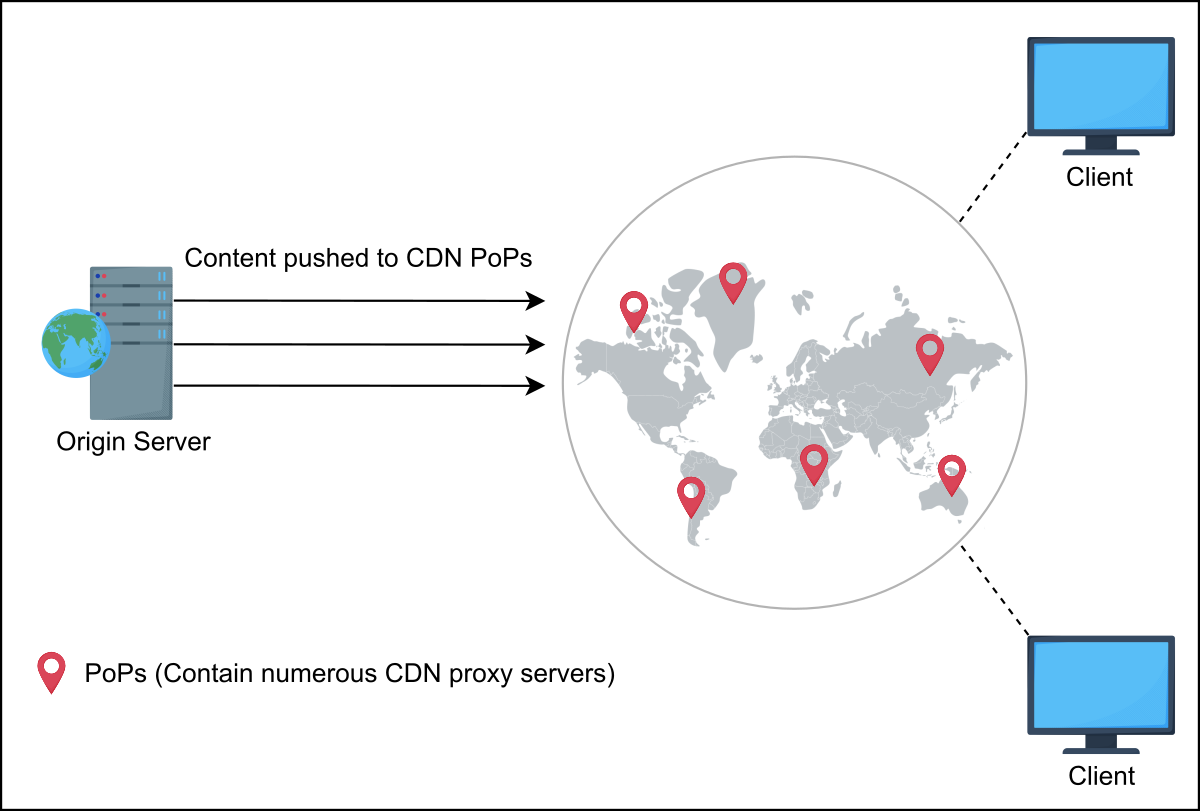
\includegraphics[width=0.5\textwidth]{Images/chapter_11/section_5267936226312192/6106868475101184.png}
 \caption{Push content to PoPs}
\end{figure}

\subsubsection{Pull CDN}\label{apBczVtf9lTUWQFFtyf4_}
\\
A CDN pulls the unavailable data from origin servers when requested by a user. The proxy servers keep the files for a specified amount of time and then remove them from the cache if they're no longer requested to balance capacity and cost.\\
\strut \\
When users request web content in the pull CDN model, the CDN itself is responsible for pulling the requested content from the origin server and serving it to the users. Therefore, this type of CDN is more suited for serving dynamic content.\\

\begin{figure}[htbp]
 \centering
 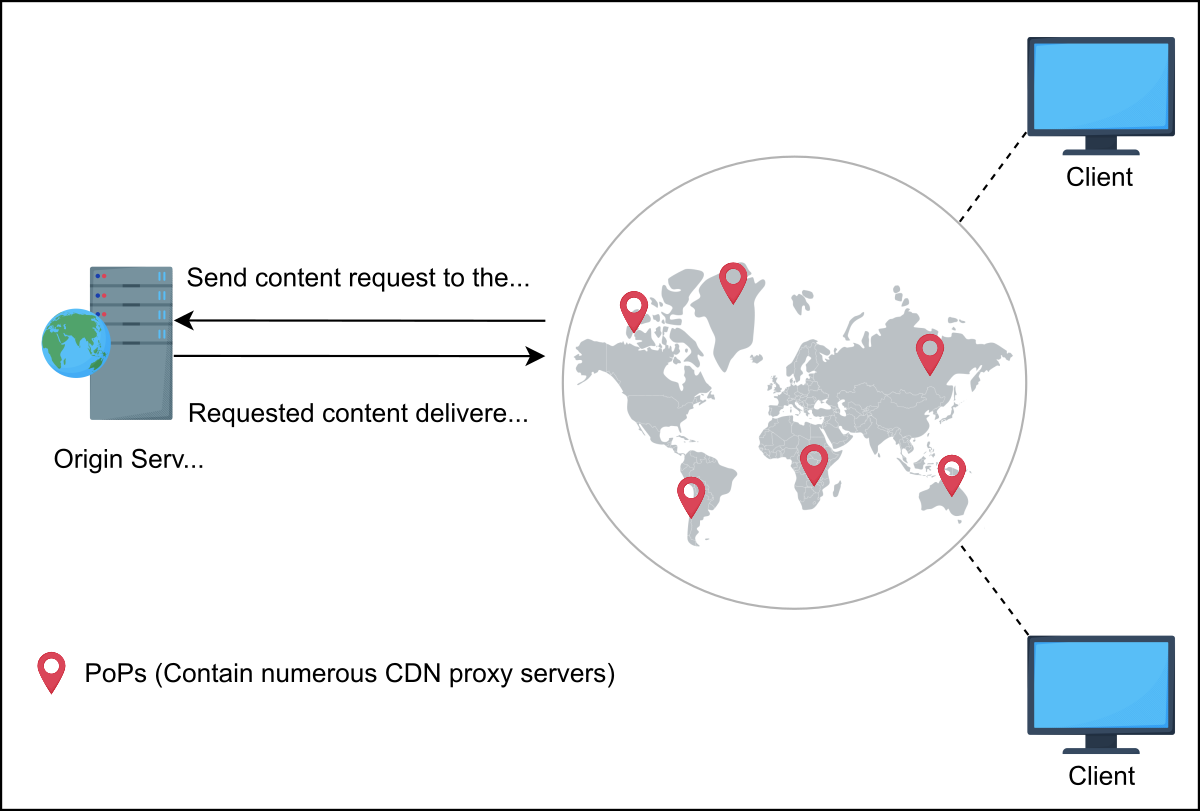
\includegraphics[width=0.5\textwidth]{Images/chapter_11/section_5267936226312192/6528393946726400.png}
 \caption{Content pull from origin server to the CDN PoPs}
\end{figure}

As stated, the push CDN is mostly used for serving static content. Since static content is served to a wide range of users for longer than dynamic content, the push CDN scheme maintains more replicas than the pull CDN, thus improving availability. On the other hand, the pull CDN is favored for frequently changing content and a high traffic load. Low storage consumption is one of the main benefits of the pull CDN.
\\
Let's say you're managing a website with two distinct content types:

\begin{itemize}
\item
\textbf{News feed:} Frequently updated articles and blog posts with varying popularity.
\item
\textbf{Static assets:} Infrequently updated items, including the company logo, website design elements, and product images.
\end{itemize}
\\
Choose between a push CDN and a pull CDN for each content type. Justify your choice.

\textbf{Question:}

Choosing between types of CDN

\textbf{Reference Answer:}

Push CDN: Static assets (logo, images) for consistent branding and fast loading. Pull CDN: News feed to handle dynamic nature and conserve storage on edge servers.

\begin{quote}
\textbf{Note:} Most content providers use both pull and push CDN caching approaches to get the benefits of both.
\end{quote}
\subsection{Dynamic content caching optimization}\label{NhqtbGhMJKcagmeJJhO4s}
\\
Since dynamic content often changes, it's a good idea to cache it optimally. This section deals with the optimization of frequently changing content.
\\
Certain dynamic content creation requires the execution of scripts that can be executed at proxy servers instead of running on the origin server. Dynamic data can be generated using various parameters, which can be beneficial if executed at the proxy servers. For example, we can generate dynamic content based on user location, time of day at a location, third-party APIs specific to a location (for instance, weather API), and so on. So , it's optimal to run the scripts at proxy servers instead of the origin servers.
\\
To reduce the communication between the origin server and proxy servers and storage requirements at proxy servers, it's useful to employ compression techniques as well. For example, Cloudflare uses Railgun to compress dynamic content.
\\
Another popular approach for dynamic data compression is \textbf{Edge Side Includes (ESI)} markup language. Usually, a small portion of the web pages changes in a certain time. It means fetching a full web page on each small change contains a lot of redundant data. To resolve this performance penalty, ESI specifies where content was changed so that the rest of the web page content can be cached. It assembles dynamic content at the CDN edge server or client browser. ESI isn't standardized yet by the World Wide Web Consortium (W3C), but many CDN providers use it.
\begin{quote}
\textbf{Note}: \textbf{Dynamic Adaptive Streaming over HTTP (DASH)} uses a manifest file with URIs of the video with different resolutions so that the client can fetch whatever is appropriate as per prevailing network and end node conditions. Netflix uses a proprietary DASH version with a Byte-range in the URL for further content request and delivery optimization.
\end{quote}
\subsection{Multi-tier CDN architecture}\label{ImLNMhw7SzfRC4-a-4FoY}
\\
The content provider sends the content to a large number of clients through a CDN. The task of distributing data to all the CDN proxy servers simultaneously is challenging and burdens the origin server significantly. CDNs follow a tree-like structure to ease the data distribution process for the origin server. The edge proxy servers have some peer servers that belong to the same hierarchy. This set of servers receives data from the parent nodes in the tree, which eventually receive data from the origin servers. The data is copied from the origin server to the proxy servers by following different paths in the tree.
\\
The tree structure for data distribution allows us to scale our system for increasing users by adding more server nodes to the tree. It also reduces the burden on the origin server for data distribution. A CDN typically has one or two tiers of proxy servers (caches). The following illustration shows the two tiers of proxy servers:

\begin{figure}[htbp]
 \centering
 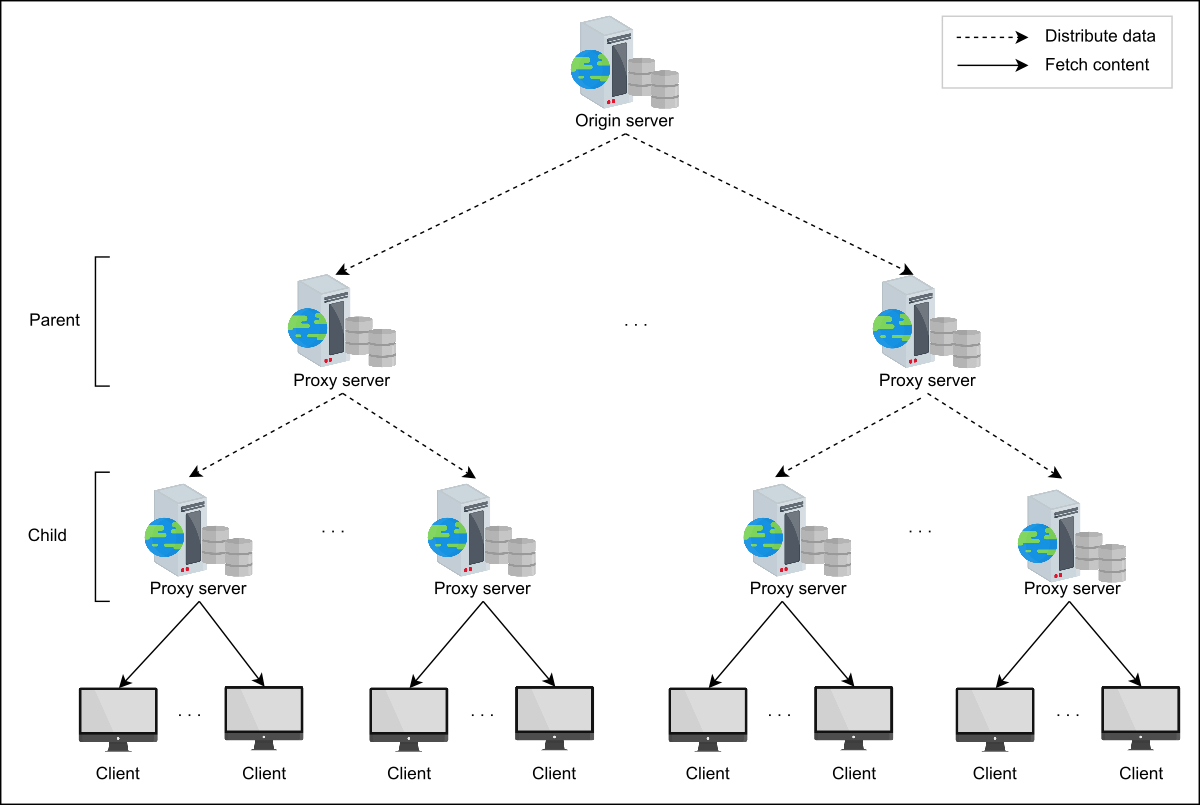
\includegraphics[width=0.3\textwidth]{Images/chapter_11/section_5267936226312192/5711479169089536.png}
 \caption{Data distribution among CDN proxy servers}
\end{figure}

Whenever a new proxy server enters the tree of a CDN, it requests the control core(The control core is a set of servers that manage the proxy servers within the PoP.), which maintains information on all the proxy servers in the CDN and provides initial content with the configuration data.
\\
Research shows that many contents have long-tail distribution. This means that, at some point, only a handful of content is very popular, and then we have a long tail of less popular content. Here, a \textbf{multi-layer cache} might be used to handle long-tail content.

\begin{figure}[htbp]
 \centering
 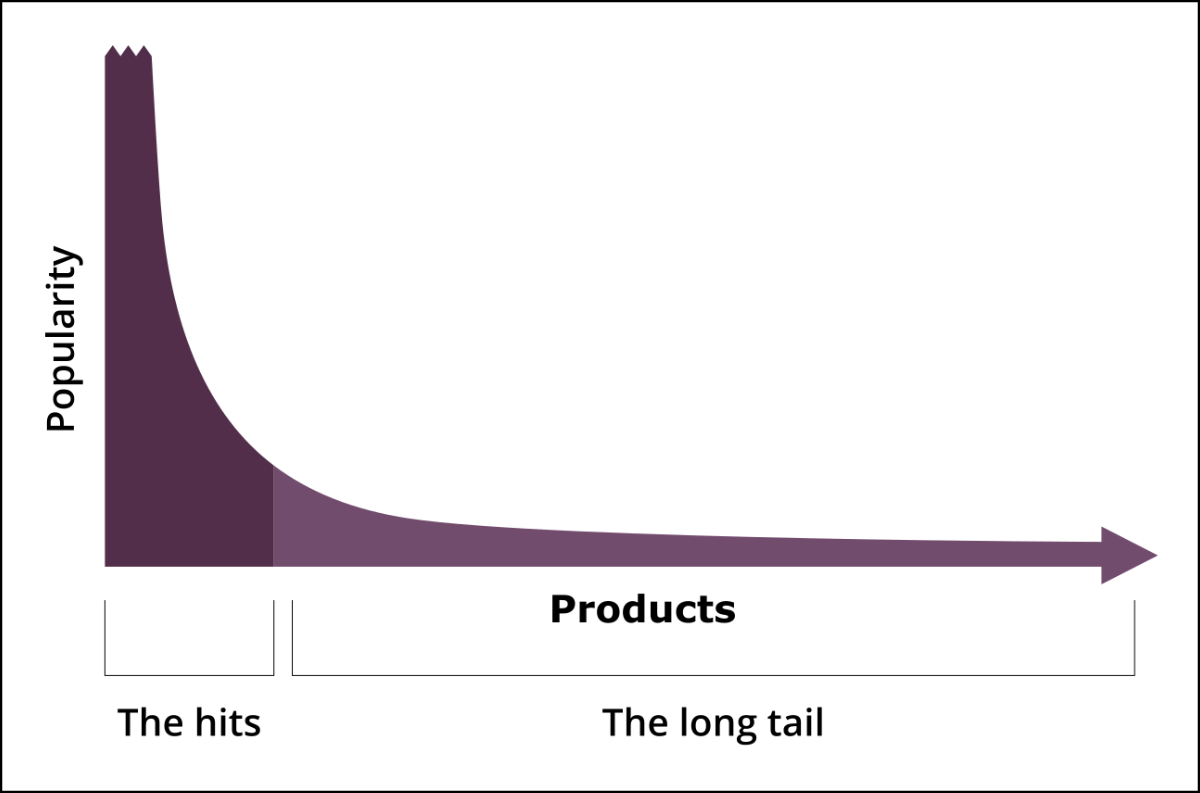
\includegraphics[width=0.3\textwidth]{Images/chapter_11/section_5267936226312192/5567677005692928.png}
 \caption{Many kinds of data exhibit the long-tailed phenomenon}
\end{figure}

\begin{quote}
\textbf{Quiz:}
\textbf{Question 1:} What happens if a child or parent proxy server fails or if the origin server fails?
\textbf{Answer:} Each PoP contains a collection of CDN proxy servers. When any child proxy server stops working due to any failures, DNS can route clients to a different child-level proxy server. Each child proxy server knows many upper-layer parent servers, and if one fails, it can go to the other one. The origin server is a set of servers with a hot backup(s), and content is in replicated store. If any of the origin servers fail, other servers take the load.
\end{quote}

Now that we've seen a way to distribute content from the origin server to all the proxy servers of the CDN, we should also educate ourselves on how users can use these proxy servers to get the data more efficiently. We 'll discuss how the nearest proxy server is chosen when clients make requests and how the CDN is located in the upcoming sections of this lesson.

\subsection{Find the nearest proxy server to fetch the data}\label{Bn1An9fsycXkC0z0epKje}
\\
It's vital for the user to fetch data from the nearest proxy server because the CDN aims to reduce user-perceived latency by bringing the data close to the user. However, the question remains of how users worldwide request data from the nearest proxy server. The goal of this section is to answer that question.

\subsubsection{Important factors that affect the proximity of the proxy server}\label{ROqNo_dtSkuSYaXNnwlaQ}
\\
There are two important factors that are relevant to finding the nearest proxy server to the user:

\begin{itemize}
\item
\protect\phantomsection\label{REXFs9FIWn7Q4Tk2w2SEp}
\textbf{Network distance} between the user and the proxy server is crucial. This is a function of the following two things:

\begin{itemize}
\item
The first is the length of the network path.
\item
The second is the capacity (bandwidth) limits along the network path.\\
The shortest network path with the highest capacity (bandwidth) is the nearest proxy server to the user in question. This path helps the user download content more quickly.
\end{itemize}
\item
\protect\phantomsection\label{ZmOma8cdbhkR-GhKSKVO-}
\textbf{Requests load} refers to the load a proxy server handles at any point in time. If a set of proxy servers are overloaded, the request routing system should forward the request to a location with a lesser load. This action balances out the proxy server load and, consequently, reduces the response latency.
\end{itemize}
\\
Let's look at the techniques that can be used to route users to the nearest proxy server.

\subsubsection{DNS redirection}\label{vaiMZomn1HJrtPGdVzM9b}
\\
In a typical \emph{DNS resolution}, we use a DNS system to get an IP against a human-readable name. However, the DNS can also return another URI (instead of an IP) to the client. Such a mechanism is called \textbf{DNS redirect}.
\\
Content providers can use DNS redirect to send a client to a specific CDN. As an example, if the client tries to resolve a name that has the word ``video'' in it, the authoritative DNS server provides another URL (for example, \protect\phantomsection\label{katex_inline_hQMv9QKMO2HCJEXgf2Ww-}{{{\(cdn.xyz.com\)}}}). The client does another DNS resolution, and the CDN's authoritative DNS provides an IP address of an appropriate CDN proxy server to fetch the required content.
\\
Depending on the location of the user, the response of the DNS can be different. Let's see the slides below to understand how DNS redirection works:

\begin{figure}[htbp]
 \centering
 \begin{subfigure}[b]{0.48\textwidth}
 \centering
 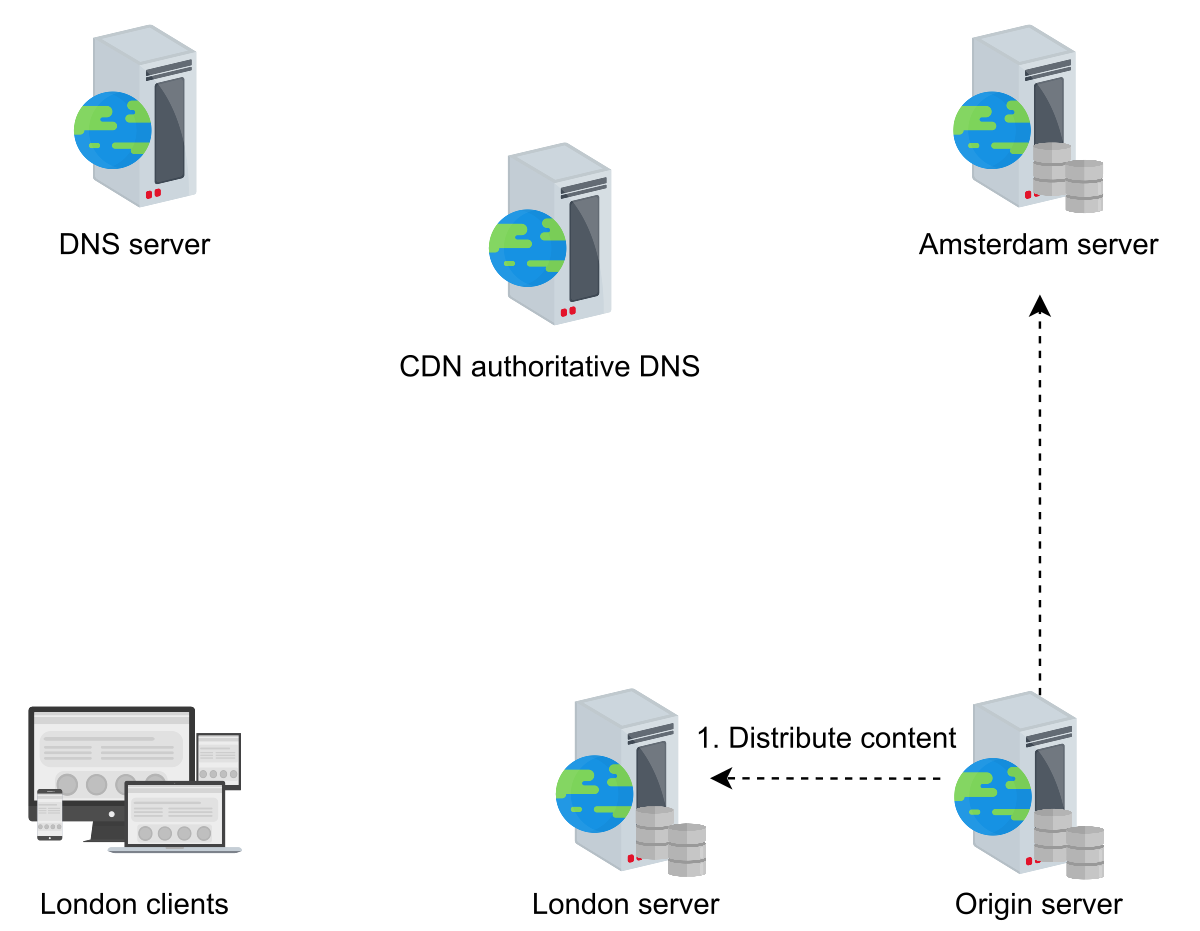
\includegraphics[width=\textwidth]{Images/chapter_11/section_5267936226312192/6586453018804224.png}
 \caption{The origin server distributes content to the London server in this example}
 \end{subfigure}
 \hfill
 \begin{subfigure}[b]{0.48\textwidth}
 \centering
 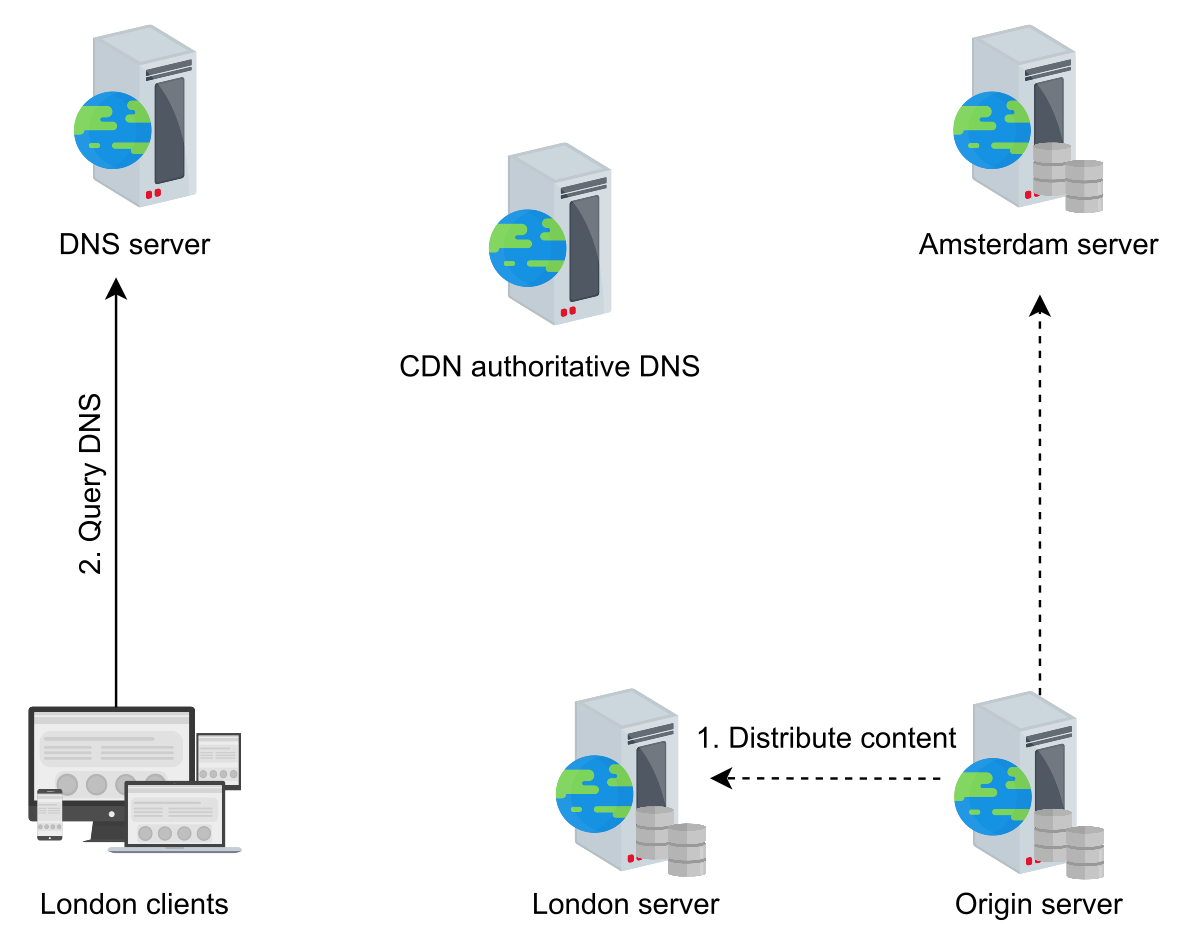
\includegraphics[width=\textwidth]{Images/chapter_11/section_5267936226312192/6335412079689728.png}
 \caption{The client requests the proxy server that’s nearest to the local DNS}
 \end{subfigure}
\end{figure}

\begin{figure}[htbp]
 \centering
 \begin{subfigure}[b]{0.48\textwidth}
 \centering
 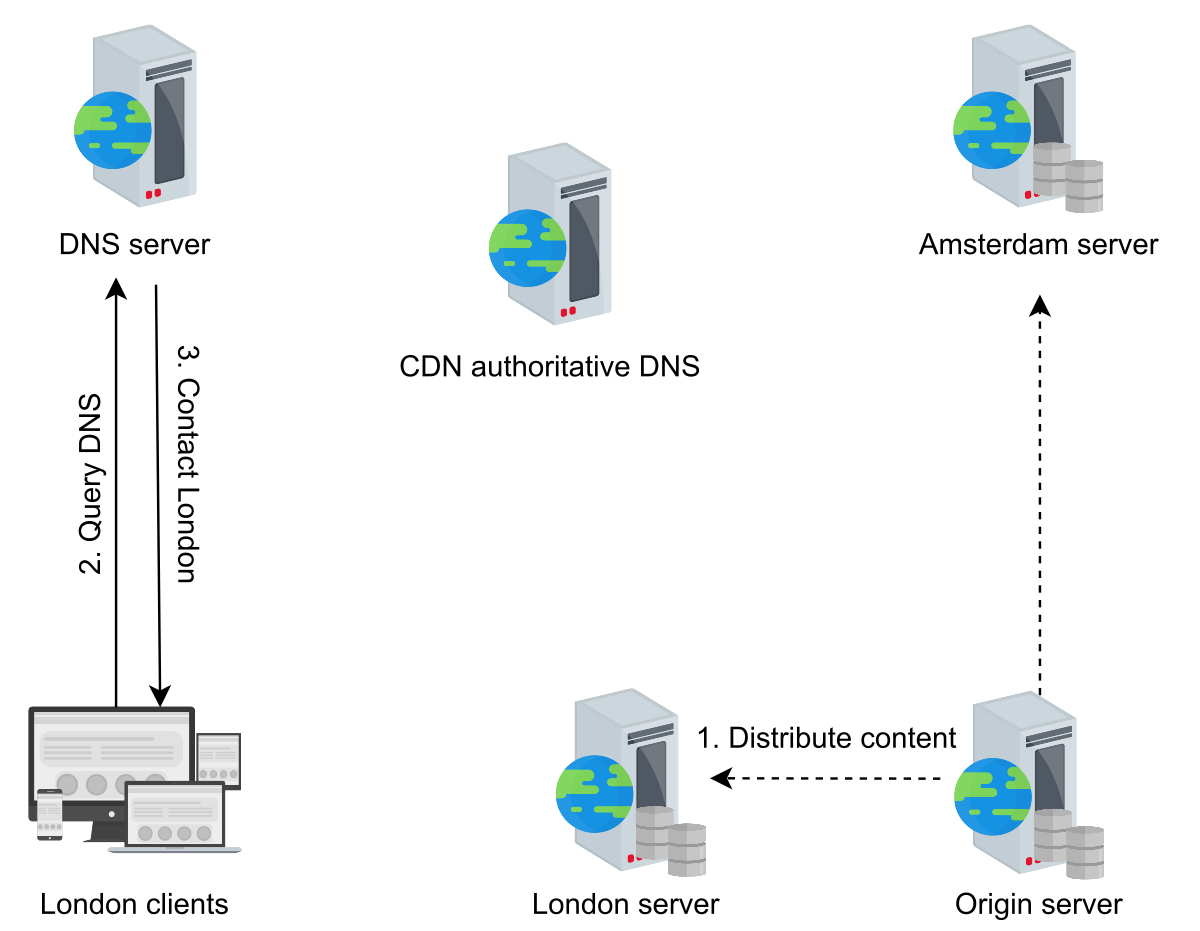
\includegraphics[width=\textwidth]{Images/chapter_11/section_5267936226312192/5816677237522432.png}
 \caption{The DNS gives the URL of the CDN authoritative DNS server to the requested clients}
 \end{subfigure}
 \hfill
 \begin{subfigure}[b]{0.48\textwidth}
 \centering
 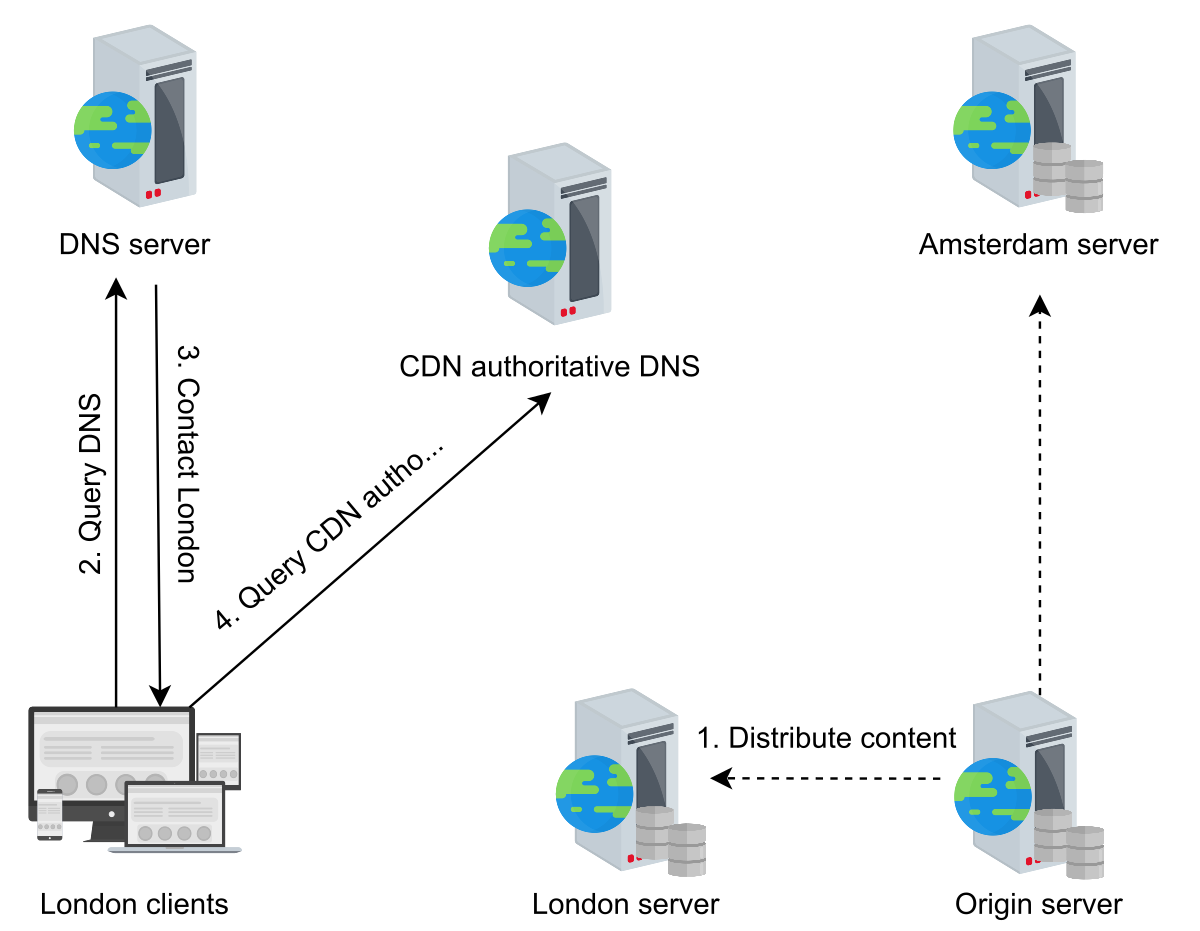
\includegraphics[width=\textwidth]{Images/chapter_11/section_5267936226312192/6209546930618368.png}
 \caption{The client requests the proxy server that’s nearest to the CDN authoritative DNS}
 \end{subfigure}
\end{figure}

\begin{figure}[htbp]
 \centering
 \begin{subfigure}[b]{0.48\textwidth}
 \centering
 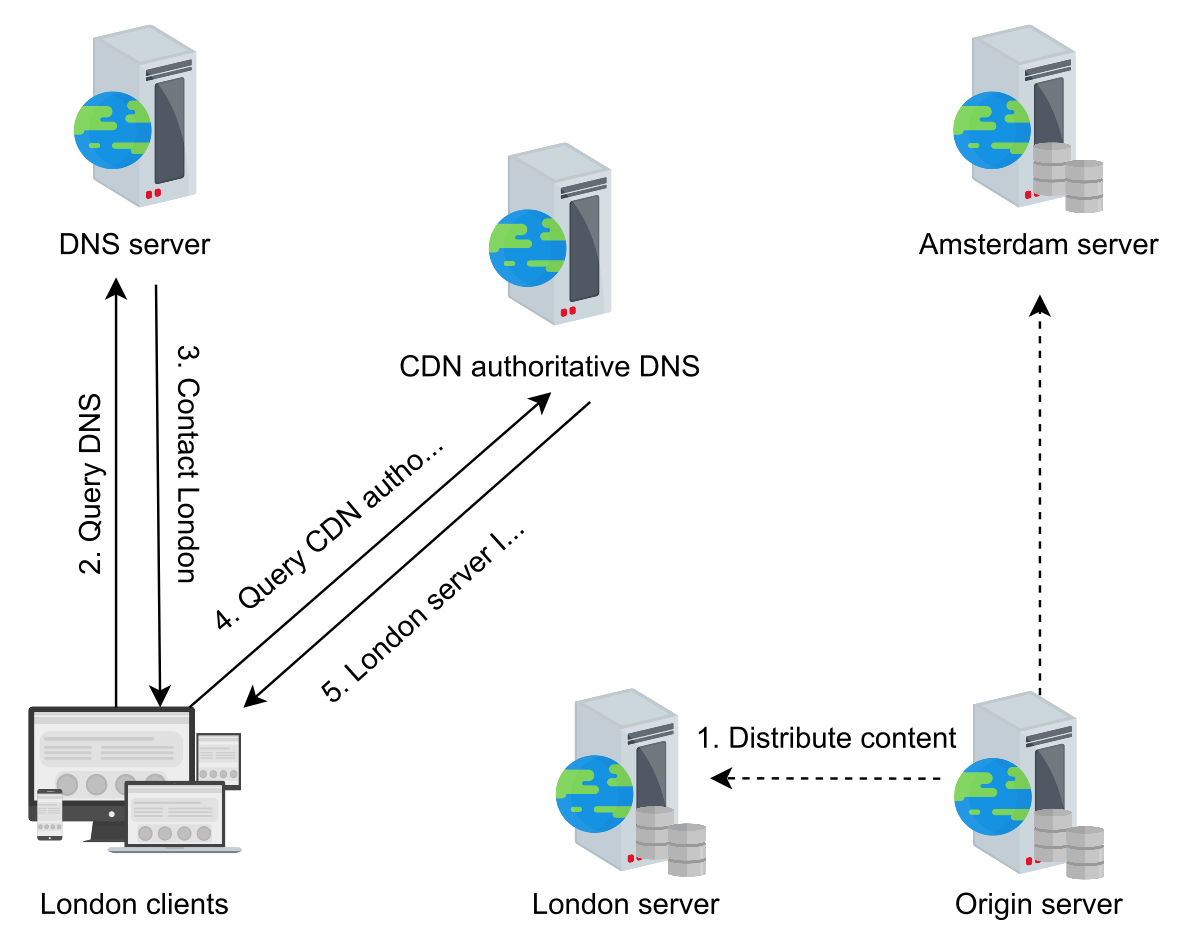
\includegraphics[width=\textwidth]{Images/chapter_11/section_5267936226312192/6559808316768256.png}
 \caption{The CDN authoritative DNS gives the IP address of the nearest proxy server to the requested clients}
 \end{subfigure}
 \hfill
 \begin{subfigure}[b]{0.48\textwidth}
 \centering
 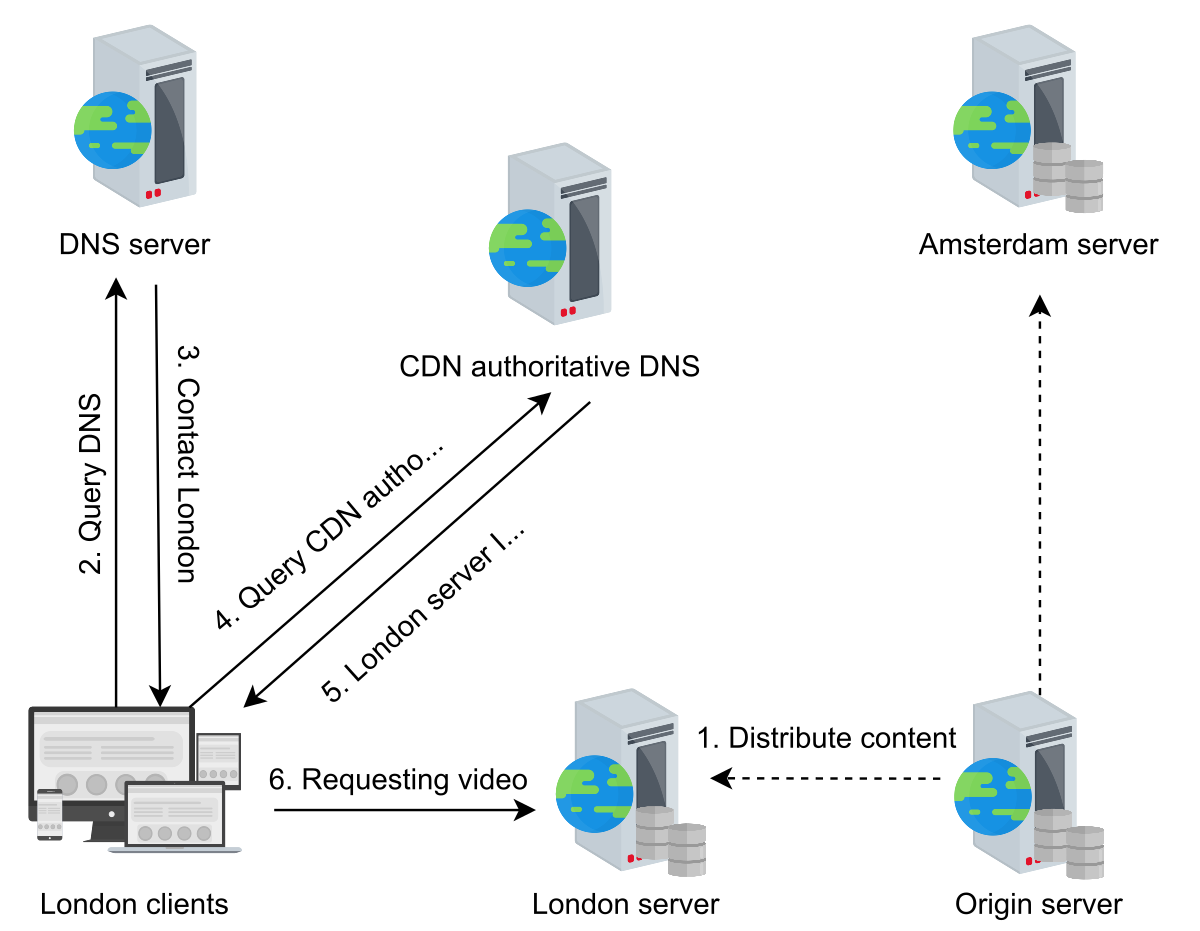
\includegraphics[width=\textwidth]{Images/chapter_11/section_5267936226312192/6178431528337408.png}
 \caption{The client requests a particular video}
 \end{subfigure}
\end{figure}

\begin{figure}[htbp]
 \centering
 \begin{subfigure}[b]{0.48\textwidth}
 \centering
 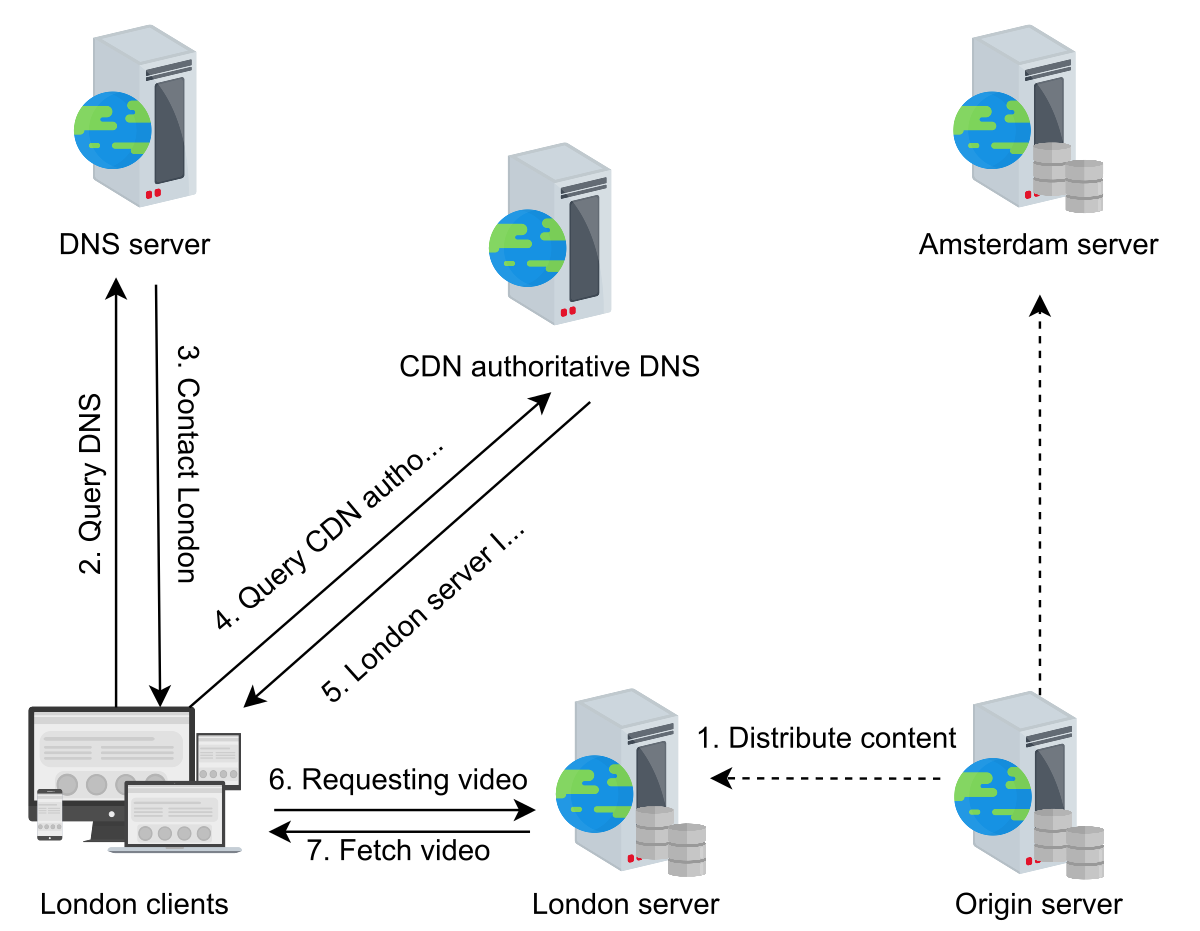
\includegraphics[width=\textwidth]{Images/chapter_11/section_5267936226312192/5988156558278656.png}
 \caption{Proxy server deliver the requested video}
 \end{subfigure}
\end{figure}

\begin{quote}
\textbf{Note}: The nearest proxy server doesn't necessarily mean the one that's geographically the closest. It could be, but it's not only the geography that matters. Other factors like network distance, bandwidth, and traffic load already on that route also matter.
\end{quote}
\\
There are two steps in the DNS redirection approach:

\begin{enumerate}
\item
\protect\phantomsection\label{6eduM93SHuDV9S2juswTM}
In the first step, it maps the clients to the appropriate network location.
\item
\protect\phantomsection\label{EvkYw-_BH-RyubHaor-Gi}
In the second step, it distributes the load over the proxy servers in that location to balance the load among the proxy servers (see \href{https://www.educative.io/courses/grokking-the-system-design-interview/introduction-to-domain-name-system-dns}{DNS} and \href{https://www.educative.io/courses/grokking-the-system-design-interview/introduction-to-load-balancers}{Load Balancers} building blocks for more details on this).
\end{enumerate}
\\
Within each location or Point of Presence (PoP), such as the London data center, intra-PoP load balancing decides which proxy server handles each incoming request. This ensures traffic is evenly distributed among local servers and maintains high availability even if one proxy becomes overloaded or temporarily unavailable.
\\
DNS redirection takes both of these important factors---network distance and requests load---into consideration, and that reduces the latency towards a proxy server.
\\
To shift a client from one machine in a cluster to another, the DNS replies at the second step are given with short TTLs so that the client repeats the resolution after a short while. DNS keeps delivering the content by routing requests to other active servers in case of hardware failures and network congestion. It does so by load balancing the traffic, using intelligent failover, and maintaining servers across many data centers, which achieves good reliability and performance.
\\
Since the load at proxy servers changes over time, the content provider needs to make appropriate changes in the DNS to make the DNS redirection effective. Many CDN providers like Akamai(Akamai was the first major CDN provider and became the industry leader.) use DNS redirection in their routing system.

\subsubsection{Anycast}\label{WAvUmtxcaVfQOUWT_opHN}
\\
\textbf{Anycast} is a routing methodology in which all the edge servers located in multiple locations share the same single IP address. It employs the \textbf{Border Gateway Protocol}(BGP is a network-level protocol used by Internet edge routers to share routing and reachability information so that every node on the network, even if independent, is aware of the status of their closest network neighbors.) \textbf{(BGP)} to route clients based on the Internet's natural network flow. A CDN provider can use the anycast mechanism so that clients are directed to the nearest proxy servers for content.

\subsubsection{Client multiplexing}\label{VS_irBHwiCt12nI3fbxTw}
\\
\textbf{Client multiplexing} involves sending a client a list of candidate servers. The client then chooses one server from the list to send the request to. This approach is inefficient because the client lacks the overall information to choose the most suitable server for their request. This may result in sending requests to an already-loaded server and experiencing higher access latency.

\subsubsection{HTTP redirection}\label{ny9eYEAZUkZ6RpxACwjnt}
\\
\textbf{HTTP redirection} is the simplest of all approaches. With this scheme, the client requests content from the origin server. The origin server responds with an HTTP protocol to redirect the user via a URL of the content.
\\
Below is an example of an HTML snippet provided by Facebook. As is highlighted in line 8, the user is redirected to the CDN to download the logo of Facebook:

\textbf{An example of HTML containing a redirection URL}

\begin{lstlisting}[language=HTML]
<!––  The code below is taken from Facebook. -->
<div class="fb_content clearfix " id="content" role="main">
 <div>
  <div class="_8esj _95k9 _8esf _8opv _8f3m _8ilg _8icx _8op_ _95ka">
   <div class="_8esk">
    <div class="_8esl">
     <div class="_8ice">
      <img class="fb_logo" src="https://static.xx.fbcdn.net/rsrc.php/y8/r/dF5SId3UHWd.svg"> 
     </div>
     <h2 class="_8eso">Facebook helps you connect and share with the people in your life.</h2>
    </div>
   </div>
\end{lstlisting}

In the next lesson, we discuss the different details of content consistency and proxy server deployment in CDN.



% End of section content